\section{Introduction}
\label{sec:intro}

Building a new chip and taking it to ``tape-out'', or the manufacturing stage, is today an extremely expensive and slow process. It involves many steps, starting from the architecture, RTL and testbench implementation at the frontend, verification, synthesis, place \& route, power optimization, and packaging and thermals analysis. All of these steps in combination result in a process that costs over \$400M and consumes 18-36 month for teams of hundreds of people (who typically start with an existing design). Any issues identified during the process can require additional design iterations, and in the worst case, ``re-spins'' of the silicon, requiring new masks.

Long-horizon autonomous AI agents present the promise of changing this paradigm. However chips, unlike software, are physical products, and this necessitates a different agent design than is optimal for coding. For one, the chip design process contains many steps spanning both logical and physical aspects, and all of these must be handled for an agent to be useful and avoid being bottlenecked. Because chips are manufactured at great upfront cost (with an N2 mask set estimated at >\$30M), functional verification takes on an even greater importance than in software. Bugs cannot be fixed by pushing a patch, and so instead painstaking efforts must be expended to ensure all cases are covered from the outset.

In our prior work \cite{team2026design}, we introduced ``Design Conductor'', a long-running multi-agent system designed to solve these problems. In that work, it was able to build a (comparatively simple) 5-stage RISC-V CPU. The agent ran for around 12 hours and used the RISC-V ISA simulator, Spike \cite{spike} as a reference model for system sim. We highlighted several limitations of Design Conductor in that work, including its architecture reasoning, understanding of timing, and need for very precise specification. In all of these regards, the Design Conductor of that time (approximately Dec. 2025) was more like a highly skilled and inexhaustible implementer than a true designer. Some in the industry also observed that openly available implementations of RISC-V cores may have been included in the pretraining data of the frontier models that Conductor uses, making the task ``easier'' for the agent to do\footnote{In the authors' opinion, this is a specious point, but we acknowledge it nonetheless.}.

\begin{figure*}[!htbp]
	\centering
	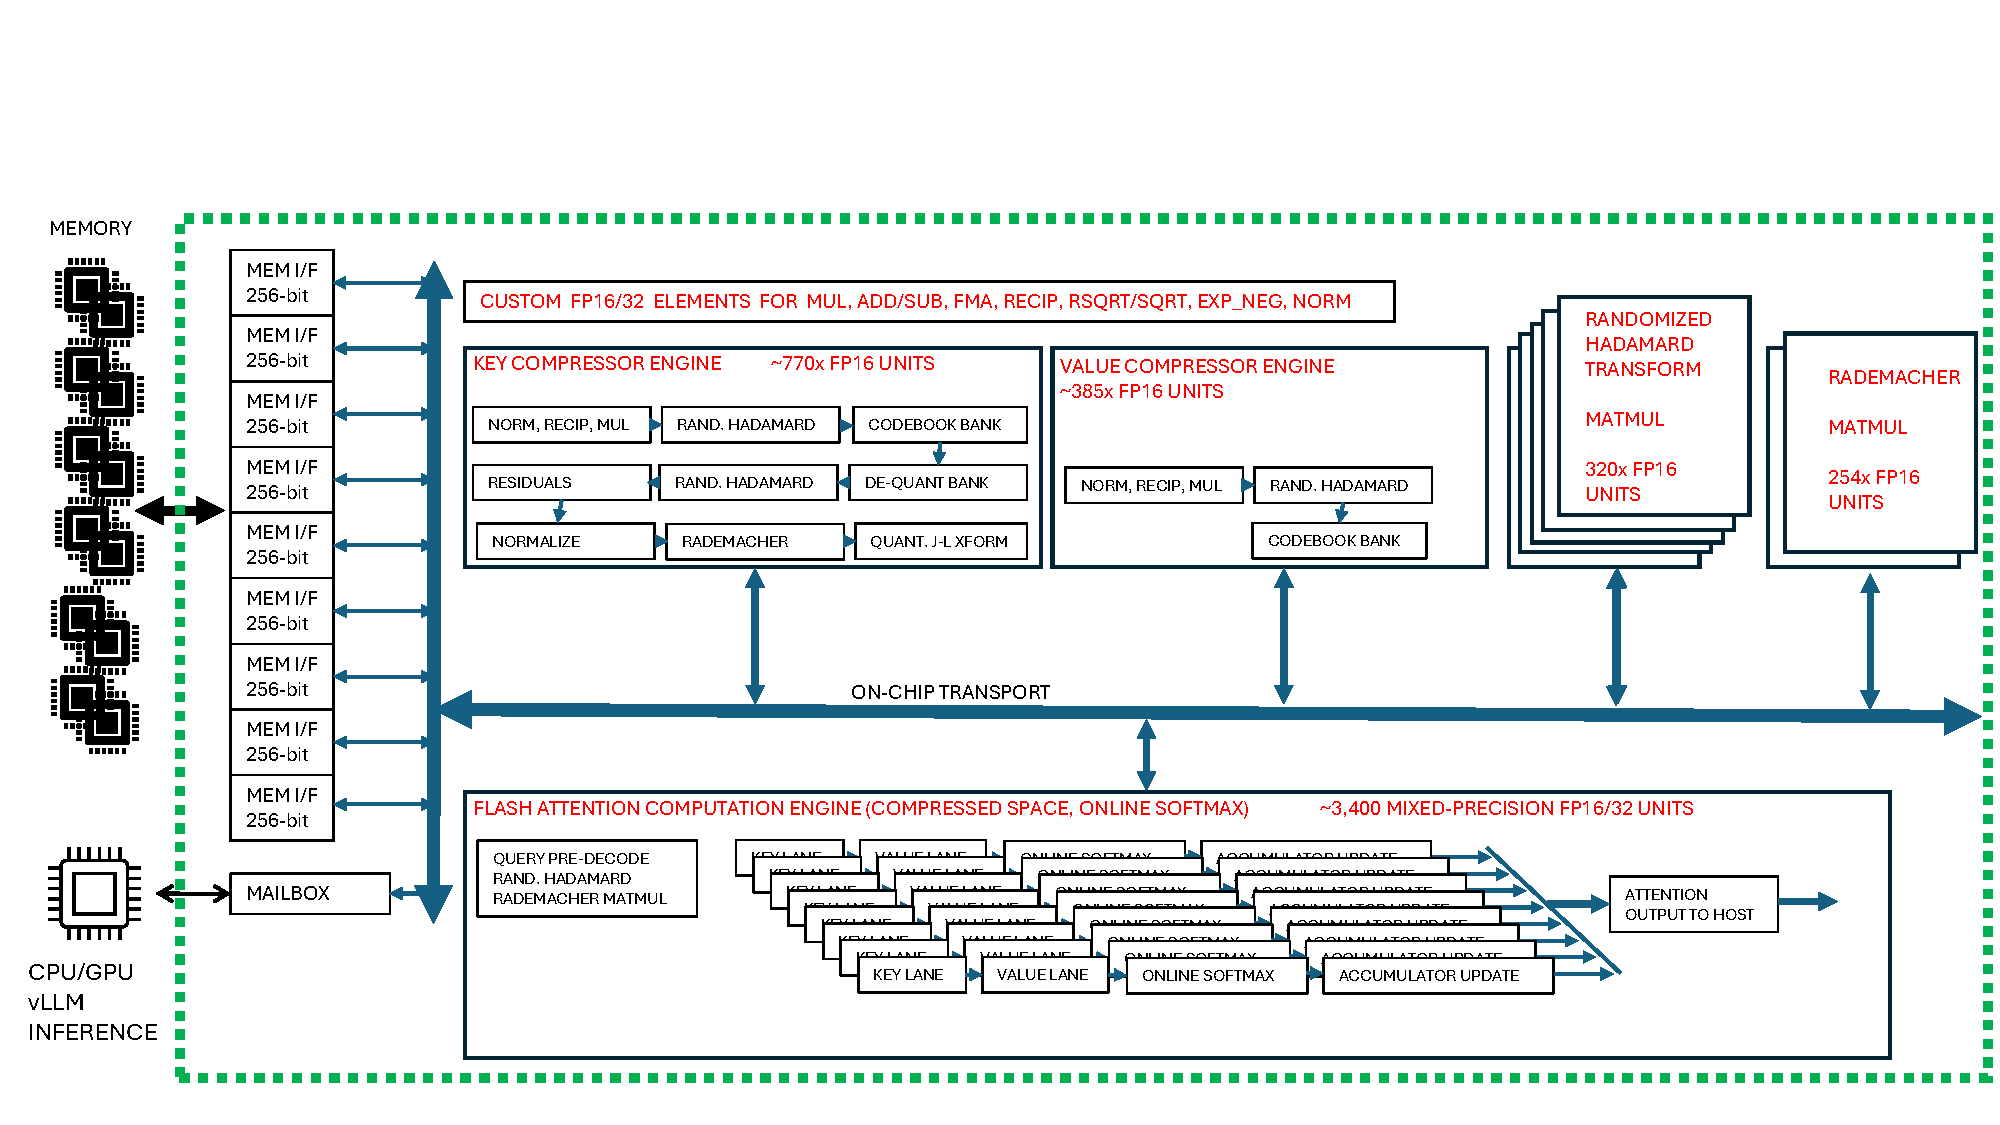
\includegraphics[width=\linewidth, trim=0.4cm 0.5cm 0cm 3.5cm, clip]{figs/VerTQ_Block_Diagram_v4.pdf}
	\caption{\textbf{``VerTQ'' TurboQuant/FlashAttention Chip by Conductor 2.0 - Block Diagram}}
	\label{fig:vertq_block}
\end{figure*}

By redesigning the Conductor harness and taking advantage of new frontier models released in April 2026, we find that the system has been able to make major inroads in each of these areas, and others. We tested this ``Design Conductor 2.0'' on many design tasks as part of our evaluation process, and we present a subset of 4 of these designs in this work. The most interesting such task was assigning Design Conductor to build ``VerTQ'', an inference accelerator for TurboQuant \cite{zandieh2025turboquant}, a KV-cache compression algorithm. It effectively architected, implemented, verified, timing-optimized, and mapped to an FPGA an accelerator for the entire LLM decode operation (both the QK and V matmuls and the online softmax) which hard-wires support for TurboQuant. To our knowledge, there is no such hardware available online (or anywhere). Figure \ref{fig:vertq_block} shows a block diagram of VerTQ.

In building VerTQ, Design Conductor demonstrated architecture judgment and the ability to guide and manage a complex project over a roughly 80-hour runtime. We believe this capability -- ``concept to layout'' -- will enable major changes in the fabless semiconductor ecosystem.